\section{Økonomi} \label{sec:dis_oekonomi}
Økonomianalysen har til formål at klarlægge mulige omkostninger og besparelser ved implementering af Fitbit Flex. I analysen estimeres disse omkostninger og besparelser, hvorfor der ud fra analysen ikke er nogen endelig konklusion på, om teknologien er omkostningseffektiv. Det vil være gavnligt med en større viden omkring sundhedsøkonomi, når det skal undersøges, hvad omkostningerne ved for lavt aktivitetsniveau for patienter med hypertension er, hvad omkostningerne ved implementering af Fitbit Flex er, samt de sundhedsmæssige gevinster ved brug af et aktivitetsarmbånd til monitorering i almen praksis. 

Da der i analysen er benyttet estimater, er der ikke blevet lavet egentlige cost-effectiveness eller cost-utility analyser. Disse ville være relevante at udarbejde, hvis værdierne for omkostninger og gevinster, i form af både vundne leveår, QALY og valuta, var mere valide. En cost-effectiveness analyse vil være værdifuld for en beslutningstagen omkring implementeringen af Fitbit Flex, da denne værdisætter omkostninger og konsekvenser af henholdsvis den subjektive monitoreringsmetode og aktivitetsarmbåndet. Yderligere vil en cost-utility analyse kunne benyttes for at fokusere på kvaliteten af vundne leveår, hvis fysisk aktivitet øger patientens livskvalitet.

Ved udarbejdelse af de førnævnte analyser vil beslutningsmatricen på \autoref{fig:cost_effect} kunne anvendes. 

\begin{table}[H]
	\centering
	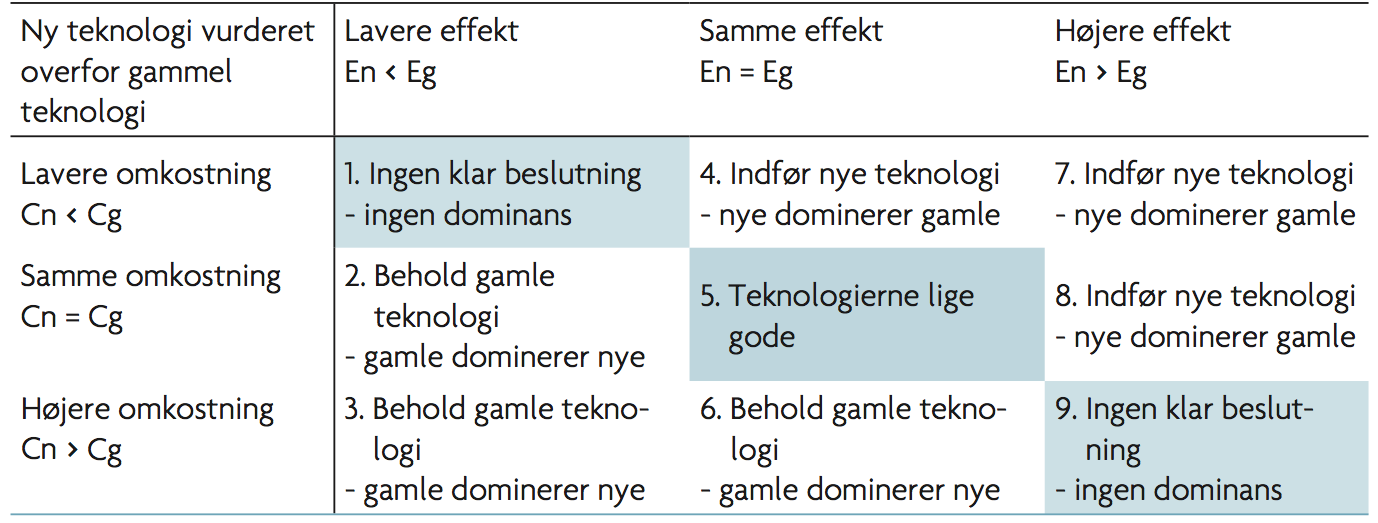
\includegraphics[width=0.9\textwidth]{figures/cost-effectiveness}
	\caption{Beslutningsmatrice ved brug af cost-effectiveness og cost-utility analyser. $E$ står for effect, men kan også benyttes til utility, og $C$ står for omkostninger. $n$ er den nye teknologi, og $g$ er den gamle \citep{mtvhaandbog}.}
	\label{fig:cost_effect}
\end{table}

\noindent
Ud fra estimaterne i økonomianalysen, vil Fitbit Flex have potentiale til at have en højere effekt end den nuværende monitoreringsmetode. De direkte omkostninger beskrevet i \autoref{sec:dir_omkost} vil være højere ved den nye teknologi, mens det er uklart, om de indirekte besparelser beskrevet i \autoref{sec:indir_omkost} er høje nok til at dække de direkte omkostninger. Hvis dette er tilfældet, vil situationen svare til beslutningsudfald 8, hvor den nye teknologi skal implementeres. Hvis omkostningerne er højere ved den nye teknologi, vil dette svare til beslutningsudfald 9, hvor der ingen klar beslutning fremgår. 